% Header
\renewcommand\evenpagerightmark{{\scshape\small Chapter 4}}
\renewcommand\oddpageleftmark{{\scshape\small Resistive Plate Chambers}}

\renewcommand{\bibname}{References}

\hyphenation{}

\chapter[Resistive Plate Chambers]%
{Resistive Plate Chambers}
\label{chapt:4}

	A \acf{RPC} is a gaseous detector using the same physical processes described in Chapter~\ref{chapt:3}. It has been developed in 1981 by Santonico and Cardarelli~\cite{SANTONICO81}, under the name of \textit{Resistive Plate Counter}, as an alternative to the local-discharge spark counters proposed in 1978 by Pestov and Fedotovich~\cite{PESTOV78,FEDOTOVICH82}. Working with spark chambers implied using high-pressure gas and high mechanical precision which the RPC simplified by formerly using a gas mixture of argon and butane flowed at atmospheric pressure and a constant and uniform electric field propagated in between two parallel electrode plates. Moreover, a significant increase in rate capability was introduced by the use of electrode plate material with high bulk resistivity, preventing the discharge from growing throughout the whole gas gap. Indeed, the effect of using resistive electrodes is that the constant electric field is locally canceled out by the development of the discharge, limiting its growth.
	
	Through its development history, different operating modes~\cite{CROTTY93,CROTTY94,CARDARELLI96} and new detector designs~\cite{ZEBALLOS96,WILLIAMS98,CZYRKOWSKI98} have been discovered, leading to further improvement of the rate capability of such a detector. Moreover, the addition of $SF_6$ into the gas mix improved the stability of operation of the RPC~\cite{CAMARRI98,ZEBALLOS98}.
	
	The low developing costs and easily achievable large detection areas offered by RPCs, as well as the wide range of possible designs, made them a natural choice to as muon chambers and/or trigger detectors in multipurpose experiments such as CMS~\cite{MUONTDR} or ATLAS~\cite{ATLASTDR}, time-of-flight detectors in ALICE~\cite{ALICETDR}, calorimeter with CALICE~\cite{CALICE2016} or even detectors for volcanic muography with ToMuVol~\cite{TOMUVOL2011}. 

\section{Principle}
\label{chapt4:sec:principle}

	RPCs are composed of two parallel resistive plate electrodes in between which a constant electric field is set. The space in between the electrodes, referred as \textit{gap}, is filled with a dense gas that is used to generate primary ionization into the gas volume. The free charge carriers (electrons and cations) created by the ionization of the gas molecules are then accelerated towards the electrodes by the electric field, as shown in Figure~\ref{fig:RPC_principle} taken from the thesis of Lippmann~\cite{LIPPMANN2003}.
	
	\begin{figure}[!h]
		\centering
		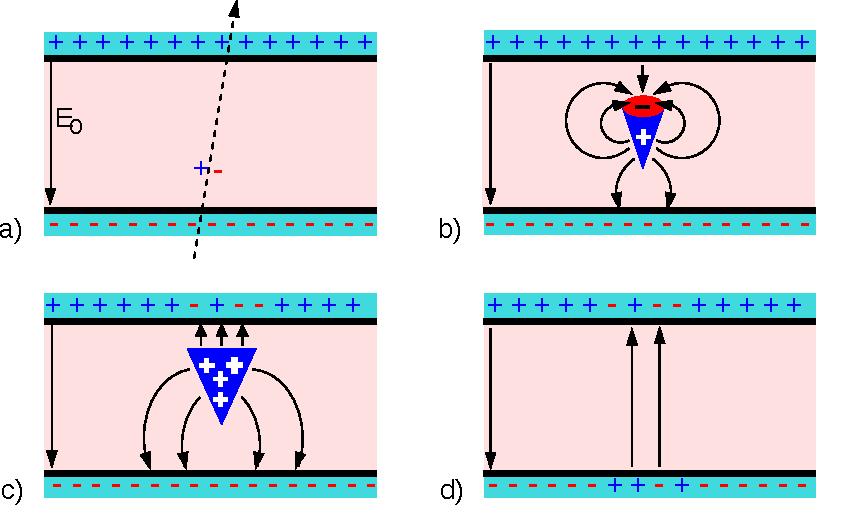
\includegraphics[width = \plotwidth]{fig/chapt4/RPC_principle.pdf}\\
		\caption{\label{fig:RPC_principle} Different phases of the avalanche development in the RPC gas volume subjected to a constant electric field $E_0$. a) An avalanche is initiated by the primary ionisation caused by the passage of a charged particle through the gas volume. b) Due to its growing size, the avalanche starts to locally influence the electric field. c) The electrons, lighter than the cations reach the anode first. d) The ions reach the cathode. While the charges have not been recombined, the electric field in the small region around the avalanche stays affected and locally blind the detector.}
	\end{figure}
	
	RPCs being passive detectors, a current on pick-up copper read-out placed outside of the gas volume is induced by the charge accumulation during the growth of the avalanche. As a result, the time resolution of the detector is substantially increased as the output signal is generated while the electrons are still in movement. The advantage of a constant electric field, over multi-wire proportional chambers, is that the electrons are being fully accelerated from the moment charge carriers are freed and feel the full strength of the electric field that doesn't depend on the distance to the readout and that the output signal doesn't need for the electrons to be physically collected.
	
	The typical gas mixture RPCs are operated with is generally composed of 3 gas compounds.
	
	\begin{itemize}
		\item[•] Tetrafluoroethane ($C_2F_4H_2$), also referred to as \textit{Freon}, is the principal compound of the RPC gas mixtures, with a typical fraction above 90\%. It is used for it's high effective Townsend coefficient and the great average fast charge that allows to operate the detector with a high threshold with respect to argon, for example, that has similar effective Townsend coefficient but suffers from a lower fast charge. To operate with similar conditions, argon would require a higher electric field leading to a higher fraction of streamers, thus limiting the rate capability of the detector~\cite{ABBRESCIA1997}.
		\item[•] Isobutane ($C_4H_10$), only present in a few percent in the gas mixtures, is used for its UV quenching properties~\cite{BATTISTONI85} helping to prevent streamers due to UV photon emission during the avalanche growth.
		\item[•] Sulfur hexafluoride, ($SF_6$), referred to simply as \textit{SF6}, is used in very little quantities for its high electronegativity. Excess of electrons are being absorbed by the compound and streamers are suppressed~\cite{ZEBALLOS98}. Nevertheless, a fraction of $SF_6$ higher than 1\% will not bring any extra benefice in terms of streamer cancelation power but will lead to higher operating voltage.
	\end{itemize}
	
	\textbf{Talk about electrodes resistivity and it's effect on charge recombination and rate capability.}

\section{Rate capability of Resistive Plate Chambers}
\label{sec:RateCapa}
	
	\subsection{Operation modes}
	\label{chapt4:ssec:operation}

\section{High time resolution}
\label{sec:TimeRes}
	
	\subsection{Electron drift velocity}
	\label{chapt4:ssec:drift}

\section{Resistive Plate Chambers at CMS}
\label{sec:CMS-RPC}

    \subsection{Overview}
    
	The Resistive Plate Chambers (RPC) system, located in both barrel and endcap regions, provides a fast, independent muon trigger with a looser p$_T$ threshold over a large portion of the pseudorapidity range ($|\eta|<1.6$) {\color{blue} [add reconstruction]}.\\
	
	During High-Luminosity LHC (HL-LHC) operations the expected conditions in terms of background and pile-up will make the identification and correct P$_T$ assignment a challenge for the Muon system. The goal of RPC upgrade is to provide additional hits to the Muon system with precise timing. All these informations  will be elaborated by the trigger system  in a global way enhancing the performance of the trigger in terms of efficiency and rate control. The RPC Upgrade is based on two projects: an improved Link Board System and the extension of the RPC coverage up to $|\eta|=2.4$. {\color{blue} [FIXME 2.4 or 2.5?]}

	The Link Board system, that will be described in section xxx, is responsible to process, synchronize and zero-suppress the signals coming from the RPC front end boards. The Link Board components have been produced between 2006 and 2007 and will be subjected to aging and failure in the long term. The upgraded Link Board system will overcome the aging problems described in section xxx and will allow for a more precise timing information to the RPC hits from 25 to \SI{1}{ns} [ref section xxx].

	The extension of the RPC system up to $|\eta|=2.1$ was already planned in the CMS TDR [ref cmstdr] and staged because of budget limitations and expected background rates higher than the rate capability of the present CMS RPCs in that region. An extensive R\&D program has been done in order to develop an improved RPC that fulfills the CMS requirements. Two new RPC layers in the innermost ring of stations 3 and 4 will be added with benefits to the  neutron-induced background reduction and efficiency improvement for both trigger and offline reconstruction.

    \subsection{The present RPC system}
    
	The RPC system is organized in 4 stations called RB1 to RB4 in the barrel region, and RE1 to RE4 in the endcap region. The innermost barrel stations, RB1 and RB2, are instrumented with 2 layers of RPCs facing the innermost (RB1in and RB2in) and outermost (RB1out and RB2out) sides of the DT chambers. Every chamber is then divided from the read-out point of view into 2 or 3 $\eta$ partitions called ``rolls''. The RPC system consist of 480 barrel chambers and 576 endcap chambers. Details on the geometry are discussed in the paper [ref to geo paper].
%A charged particle crossing an RPC will ionize the gas in both gas volumes and the avalanches generated by the high electric field will induce an image charge, which is picked up by the readout strips. 
%This signal is discriminated and shaped by the front-end electronics placed on the detector.
%In the endcaps, each station is divided into 3 rings (identified as rings 1, 2, and 3) at increasing radial distance from the beam line.
%Up to now the ring 1 was never instrumented; the RPC system therefore covered only the region up to $\eta$ = 1.6. 
%Each endcap ring is composed of 36 chambers covering the full azimuthal range. 
%From the readout point of view, each endcap chamber is divided into 3 $\eta$ partitions (rolls) identified by the letters A, B, and C. Thus the endcap RPCs are identified in the following way: 
%REn/r/x where n is the station ($\pm$1, $\pm$2, $\pm$3), r is the ring (2 or 3), and x is the roll (A, B, or C).

	The CMS RPC chamber is a double-gap, operated in avalanche mode to ensure reliable operation at high rates. Each RPC gap consists of two 2-mm-thick resistive High-Pressure Laminate (HPL) plates separated by a 2-mm-thick gas gap. The outer surface of the HPL plates is coated with a thin conductive graphite layer, and a voltage is applied. The RPCs are operated with a 3-component, non-flammable gas mixture consisting of 95.2$\%$ freon (C$_2$H$_2$F$_4$, known as R134a), 4.5$\%$ isobutane (i-C$_4$H$_{10}$), and 0.3$\%$  sulphur hexafluoride (SF$_6$) with a relative humidity of 40$\%$ - 50$\%$. Readout strips are aligned in $\eta$ between the 2 gas gaps. {\color{blue} [Add a sentence on FEBs.]}

	The discriminated signals coming from the Front End boards feed via twisted cables (10 to \SI{20}{m} long) the Link Board System located in UXC on the balconies around the detector. The Link System consist of the 1376 Link Boards (LBs) and the 216 Control Boards (CBs), placed in 108 Link Boxes. The Link Box is a custom crate (6U high) with 20 slots (for two CBs and eighteen LBs). The Link Box contains custom backplane to which the cables from the chambers are connected, as well as the cables providing the LBs and CBs power supply and the cables for the RPC FEBs control with use of the I2C protocol (trough the CB). The backplane itself contains only connectors (and no any other electronic devices).

	The Link Board has 96 input channels (one channel corresponds to one RPC strip). The input signals are the $\sim$\SI{100}{ns} binary pulses which are synchronous to the RPC hits, but not to the LHC clock (which drives the entire CMS electronics). Thus the first step of the FEB signals processing is synchronization, i.e. assignment of the signals to the BXes (\SI{25}{ns} periods). Then the data are compressed with a simple zero-suppressing algorithm (the input channels are grouped into 8 bit partitions, only the partitions with at least one nonzero bit are selected for each BX). Next, the non-empty partitions are time-multiplexed i.e. if there are more than one such partition in a given BX, they are sent one-by-one in consecutive BXes. The data from 3 neighbouring LBs are concentrated by the middle LB which contains the optical transmitter for sending them to the USC over a fiber 
at \SI{1.6}{Gbps}.

	The Control Boards provide the communication of the control software with the LBs via the FEC/CCU system. The CBs are connected into token rings, each ring consists of 12 CBs of one detector tower and a FEC mezzanine board placed on the CCS board located in the VME crate in the USC. In total, there are 18 rings in the entire Link System. The CBs also perform automatic reloading of the LB's firmware which is needed in order to avoid accumulation of the radiation induced SEUs in the LBs firmware. 

	Both LBs and CB are based on the Xilinx Spartan III FPGAs, the CB additionally contains radiation-tolerant (FLASH based) FPGA Actel ProAsicPlus.

	The High Voltage power system is located in USC, not exposed to radiation and easily accessible for any reparation. A single HV channel powers 2 RPC chambers both in the barrel and endcap regions. The Low Voltage boards are located in UXC on the balconies and provide the voltage to the front end electronics.

    \subsection{Pulse processing of CMS RPCs}
    \label{ssec:PulseProc}
	
		Signals induced by cosmic particle in the RPC strips are shaped by standard CMS RPC \acf{FEE} following the scheme of Figure~\ref{fig:DAQ}. On a first stage, analogic signals are amplified and then sent to the \acf{CFD} described in Figure~\ref{fig:CFD}. At the end of the chain, \SI{100}{ns} long pulses are sent in the LVDS output. These output signal are sent on one side to a V1190A \acf{TDC} module from CAEN and on the other to an OR module to count the number of detected signals. Trigger and hit coïncidences are monitored using scalers. The TDC is used to store the data into ROOT files. These files are thus analysed to understand the detectors performance.

			\begin{figure}[!h]
			\begin{subfigure}{\linewidth}
				\centering
				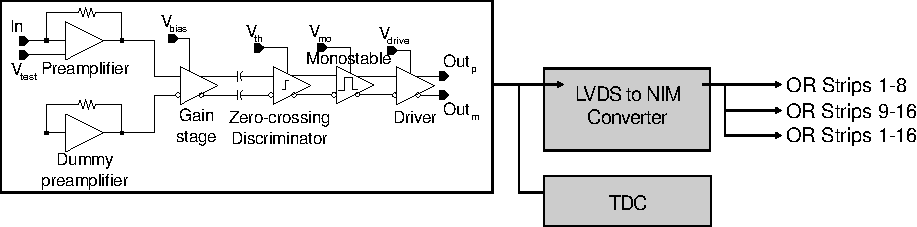
\includegraphics[width = \plotwidth]{fig/chapt5/pulse-processing.pdf}\\
				\caption{\label{fig:DAQ:A}}
			\end{subfigure}
			\begin{subfigure}{\linewidth}
				\centering
				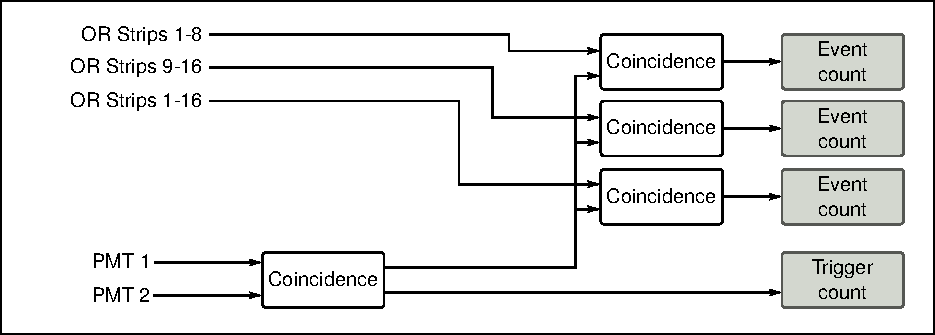
\includegraphics[width = \plotwidth]{fig/chapt5/pulse-processing-2.pdf}
				\caption{\label{fig:DAQ:B}}
			\end{subfigure}
			\caption{\label{fig:DAQ} Signals from the RPC strips are shaped by the FEE described on Figure ~\ref{fig:DAQ:A}. Output LVDS signals are then read-out by a TDC module connected to a computer or converted into NIM and sent to scalers. Figure~\ref{fig:DAQ:B} describes how these converted signals are put in coincidence with the trigger.}
		\end{figure}
		
		\begin{figure}[!h]
			\begin{subfigure}{\linewidth}
				\centering
				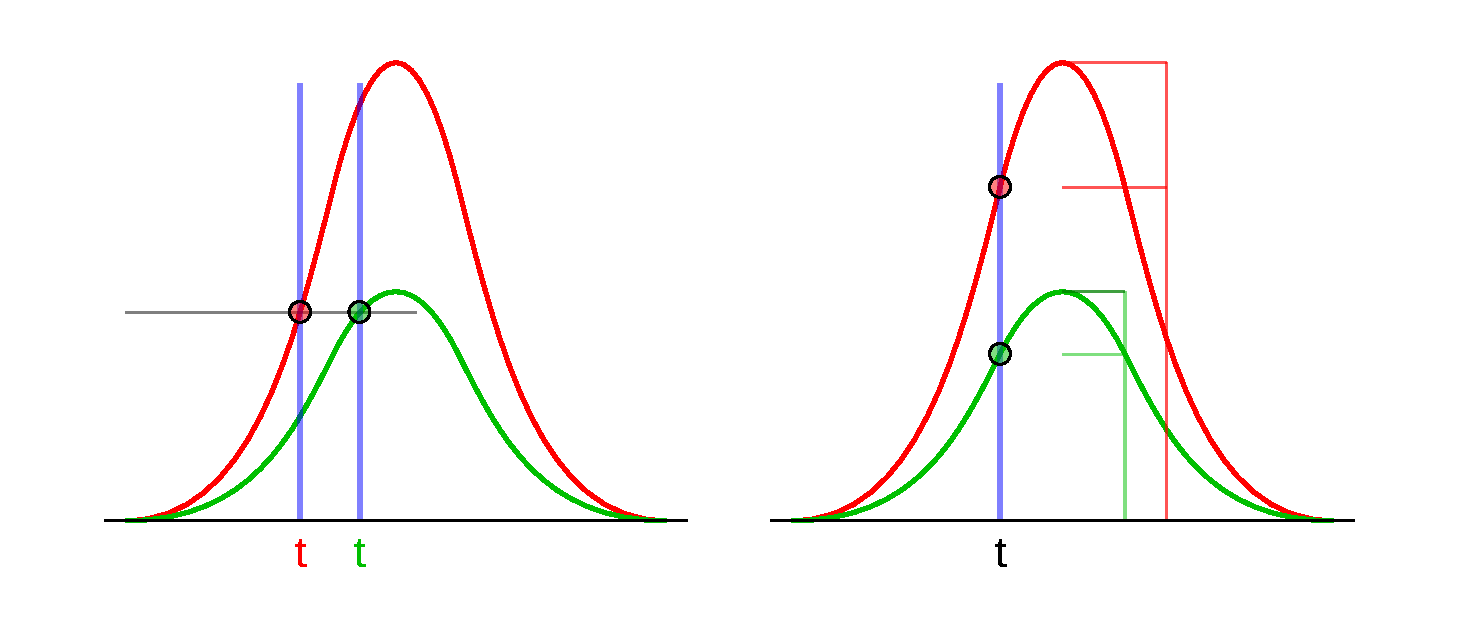
\includegraphics[width = \plotwidth]{fig/chapt5/CFD_1.pdf}\\
				\caption{\label{fig:CFD:A}}
			\end{subfigure}
			\begin{subfigure}{\linewidth}
			    \centering
				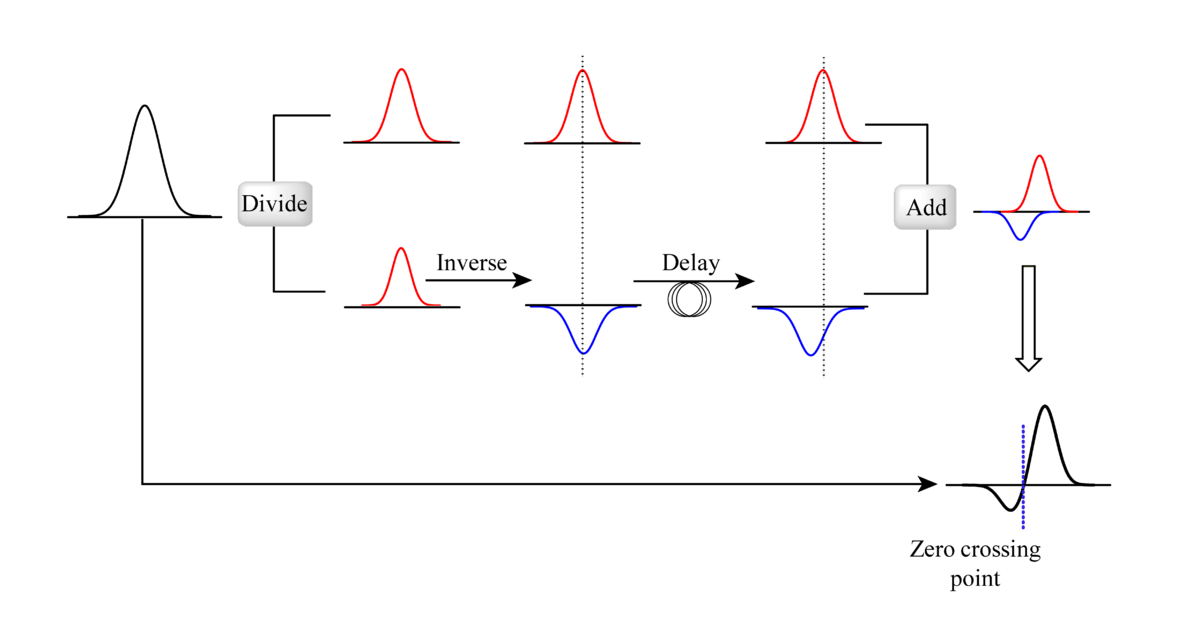
\includegraphics[width = 1.2\plotwidth]{fig/chapt5/CFD_2.png}
				\caption{\label{fig:CFD:B}}
			\end{subfigure}
			\caption{\label{fig:CFD} Description of the principle of a CFD. A comparison of threshold triggering (left) and constant franction triggering (right) is shown in Figure~\ref{fig:CFD:A}. Constant franction triggering is obtained thanks to zero-crossing technique as explained in Figure~\ref{fig:CFD:B}. The signal arriving at the input of the CFD is split into three components. A first one is delayed and connected to the inverting input of a first comparator. A second component is connected to the noninverting input of this first comparator. A third component is connected to the noninverting input of another comparator along with a threshold value connected to the inverting input. Finally, the output of both comparators is fed through an AND gate.}
		\end{figure}

\clearpage{\pagestyle{empty}\cleardoublepage}
